\documentclass[12pt,a4paper,oneside]{book}
\usepackage{amsmath}
\usepackage{amssymb}
\usepackage{amsthm}
\usepackage{graphicx}
\usepackage{latexsym}
%\usepackage{pslatex}
\usepackage{caption, booktabs}
\usepackage{color}
\usepackage{fancyhdr}
\usepackage{cite}
\usepackage{indentfirst}
\usepackage{tocloft}
\usepackage{multirow}
\usepackage{fontspec}
\usepackage{longtable}
\usepackage[german]{babel}
% Times New Roman
\setromanfont[
BoldFont=Times New Roman Bold.ttf,
ItalicFont=Times New Roman Italic.ttf,
BoldItalicFont=Times New Roman Bold Italic.ttf,
]{Times New Roman.ttf}
%\setmainfont{Times New Roman}

% Centering Chapter
\usepackage{sectsty}   
\chapterfont{\centering}

\pagestyle{myheadings}
\setlength{\parindent}{0.8in}

\usepackage[top=1.5in,bottom=1in,left=1.5in,right=1in]{geometry}

% Dient zum Verlinken der Inhaltsverzeichnisteile zu den einzelnen Seiten
\usepackage[colorlinks,
    pdfpagelabels,
    pdfstartview = FitH,
    bookmarksopen = true,
    bookmarksnumbered = true,
    linkcolor = black,
    urlcolor = cyan,
    plainpages = false,
    hypertexnames = false,
    citecolor = black
]{hyperref}

\hypersetup{
    pdftitle={MechaWars}
}

% Theorem style-------------------------------------------------------------------
\theoremstyle{plain}
\newtheorem{thm}{Theorem}[chapter]
\newtheorem{lem}[thm]{Lemma}
\newtheorem{cor}[thm]{Corollary}
\newtheorem{prop}[thm]{Proposition}
\newtheorem{rem}[thm]{Remark}
\newtheorem{ex}[thm]{Example}
\newtheorem{de}[thm]{Definition}
\renewcommand{\proof}{\textbf{Proof.}}

\numberwithin{equation}{chapter} \DeclareMathOperator{\Var}{Var}
\DeclareMathOperator{\Ima}{Im}

\usepackage{float}
%\usepackage[skip=2pt,font=footnotesize]{caption}

% Graph-------------------------------------------------------------------
\usepackage{graphics,graphicx}
\usepackage{calc}
\usepackage{tikz}
\usetikzlibrary{decorations.markings}
\tikzstyle{vertex}=[circle, draw, inner sep=2pt, minimum size=4pt]
\newcommand{\vertex}{\node[vertex]}
\newcounter{Angle}

% Line space-------------------------------------------------------------------
\renewcommand{\baselinestretch}{1.5}

\newcommand*{\QEDA}{\hfill\ensuremath{\large{\lozenge}}}
\newcommand*{\QEDAa}{\hfill\ensuremath{\square}}

\renewcommand{\bibname}{\centerline{\Large REFERENCES}}

%Centering table of contents and list of table
\usepackage{tocloft}
\renewcommand{\contentsname}{\hfill\bfseries\Large Inhaltsverzeichnis \hfill}   
\renewcommand{\cftaftertoctitle}{\hfill}





\begin{document}
\thispagestyle{empty}

\begin{center}
\large{\textbf{MechaWars\\-\\RoboRally in Java programmiert.}}
\end{center}

\vskip2.5cm

\begin{center}
\textbf{Handbuch erstellt von}
\end{center}

\vskip0.6cm

\begin{center}
\textbf{Tim Michael Kretzschmar}\\
\textbf{(mit freundlicher Unterstützung von Marc André Uxa)}

\end{center}

%\begin{figure}[h!]
%\vskip1in
%\begin{center}
%\includegraphics[width = 11 cm]{Startbildschirm.png}
%\end{center}
%\end{figure}

\vskip0.5cm
 
\begin{center}
\textbf{Software-Projekt des Jahrgangs 19INB der HTWK Leipzig}
\end{center}


%\newpage
\section*{}
\newpage

%\pagenumbering{roman}
%\addcontentsline{toc}{chapter}{LIST OF TABLES}
\tableofcontents
%


\newpage
\pagenumbering{arabic}
\chapter{Einleitung}

% Beginn Text
   
    \newpage
% Ende Text


\chapter{Die Packages}
\section{htwk.mechawars}
\hypertarget{ConfigReader.java}{}
\subsection{ConfigReader.java}
    %
    In dieser Klasse werden alle Grundeinstellungen aus der "config"-Datei eingelesen und in Variablen gespeichert, welche alle über Getter-Funktionen verfügen und somit für den Programmablauf verfügbar gestellt werden. \\
    Da man die Spieler-Anzahl ändern kann z.B. existiert eine Funktion, um diese Anzahl in der "Startupconfig.txt" zu manipulieren.
    %

\hypertarget{GameOverScreen.java}{} 
\subsection{GameOverScreen.java}
    %
    Dies ist der Bildschirm, welcher erscheint, wenn man verliert. Dabei besteht dort die Möglichkeit, wieder zum \hyperlink{MainMenue.java}{\textit{Startbildschirm/Hauptmenü}} zurückzukehren oder das Spiel zu beenden.
    %
    
\hypertarget{MainMenue.java}{}
\subsection{MainMenue.java}
    %
    Hier wird die GUI (Graphical User Interface $\widehat{=}$ Graphische Benutzeroberfläche) für den Startbildschirm verwaltet. So sind z.B. im Konstruktor die zwei Buttons hier gelistet mit ihren Funktionen - Weiter zum Auswahlbildschirm und Beenden des Spiels. \\
    Ebenfalls wir hier in Zeile 32 der Hintergrund festgelegt, welcher in Zeile 102 dann gerendert wird in der von LibGDX mitgelieferten \textt{render(float delta)}-Funktion. \\
    Die Klasse implementiert \textit{Screen} von LibGDX, womit als Interface eine ganze Menge Funktionen eingebunden werden, die jedoch zum großen Teil unverändert dastehen. Somit also von LibGDX selbst verwaltet/standartisierd sind.
    %
    
\subsection{MechaWars.java}
    %
    Diese Klasse \textit{extends Game}, ist also von der LibGDX Klasse abhängig. \\
    Besonderes Augenmerk sollte man der \texttt{create()}-Funktion widmen. Dort wird der \hyperlink{ConfigReader.java}{\textit{ConfigReader}} aufgerufen und anschließend überprüft, ob der \hyperlink{MainMenue.java}{\textit{Startbildschirm}} aufgerufen werden soll, oder sofort das Spiel mit den Grundeinstellungen gestartet wird..
    %

\subsection{OptionScreen.java}
    %
    Dieser Bildschirm ist eine umfangreiche Einstellmöglichkeit im Spiel. Hier ist auswählbar ob man im Tainingsmodus oder normalen Spielmodus starten möchte. Ebenfalls die Anzahl der rivalisierenden Roboter und die gewünschte Karte ist hier auswählbar. Sollte keine Map eingetragen sein, so spielt man mit der als Standart hinterlegten Karte.
    %
  
\subsection{VictoryScreen.java}
    %
    Das Pandon zum \hyperlink{GameOverScreen.java}{\textit{GameOverScreen.java}}.
    Dieser Bildschirm erscheint, wenn man gewinnt. Dabei besteht dor die Möglichkeit, wieder zum \hyperlink{MainMenue.java}{\textit{Startbildschirm/Hauptmenü}} zurückzukehren oder das Spiel zu beenden.
    %
    

\newpage
\section{htwk.mechawars.ai}
\subsection{AiCardGeneration.java}
    %
    Für den KI-Mitspieler werden hier der LinkedList<Card> Karten herausgenommen und zurück-übergegeben.
    %
    
\subsection{AiInterface.java (Interface)}
    %  
    Dieses Interface organisiert alle KI-Klassen, so dass sie eine Menge an Roboter haben, ein Board und die Funktion \textt{generateCards()}.
    %
    
\subsection{AiManager.java}
    %
    Hier werden alle KI (-Objekte) verwaltet. Import und Export (Speichern) erfolgen ebenfalls hier.
    %


\newpage
\section{htwk.mechawars.board}
\subsection{Board.java}
    %
    In dieser Klasse wird das Spielfeld als board (engl. = (Spiel-)Brett) angelegt. Dazu gibt es dort beim Erstellen die Pflicht, einen String, ursprünglich aus einer Datei, als Einträge zu übergeben. Diese werden dort dann interpretiert und auf Fehler wie zu lang oder zu kurz überprüft.\\
    Über die \texttt{toString}-Funktion kann das aktuelle Board als String wieder ausgelesen werden.\\
    Weiterhin wird hier das Bewegen eines Roboters über die \texttt{move}-Funktion ausgeführt.\\
    Es finden sich noch weitere Funktionen, deren Funktionalität über den Funktionen als Kommentar nachzulesen sind, wie der Laser-Check z.B.
    %
    
\hypertarget{Dir.java}{}
\subsection{Dir.java (Enumeration)}
    %
    Eine Enumeration für die Codierung der Richtung eines Roboters. Dabei gibt es eine \texttt{North} (Norden), \texttt{East} (Osten), \texttt{South} (Süden) und \texttt{West} (Westen). Dies wird als Integer-Wert abgespeichert und über die dazu erstellte Funktion \textit{intToDirection()} dann als \texttt{Dir} zurückgegeben bei Aufruf oder Bedarf.
    %
    
\subsection{Robot.java}
    %
    Diese Klasse beschreibt einen Roboter. In ihr werden essentielle Attribute gespeichert, auszugsweise wären das die Richtung des Roboters (\hyperlink{Dir.java}{\textit{dir}}), die aktuelle Position (\texttt{xcoor} und \texttt{ycoor}), die Lebenspunkte (\texttt{damagePoints}) oder der aktuelle Zerstörungsstatus (boolean \texttt{destroyed}). \\
    Es gibt noch eine Funktion neben dem Konstruktor, der die übergebene Anzahl an Robotern erstellt, als Robot[]-Array. \\
    Die Bewegung des Roboters wird ebenfalls hier definiert, genauso wie eine Drehung abzulaufen hat. \\
    Neben den ganzen Getter- und Setter-Funktionen gibt es auch noch weitere Funktionen, wie die \textit{addCard()}-Funktion um eine weitere \hyperlink{Card.java}{\textit{Karte}} hinzuzufügen.
    %

\newpage
\section{htwk.mechawars.cards}
\hypertarget{Card.java}{}
\subsection{Card.java}
    %
    Diese Klasse enthält das Gerüst für Karten. Deshalb sind dort die drei Attribute \texttt{cardAttributeType}, \texttt{cardAttributeMovCount} und \texttt{cardAttributePriority} angelegt. \\
    Das erste beschreibt als Enumeration die Art der Karte (\hyperlink{Type.java}{siehe \textit{Type.java}}) \\
    Das zweite Attribut dagegen ist ein "byte" und sagt aus, wie viele Bewegungen der Art ausgeführt werden sollen. Dies ist durch folgende Tabelle codiert: \\
    \begin{center} \begin{longtable}{|l|c|l|}
    \hline
    \textit{byte}   & \textit{mov (Bewegung)}           & \textit{turn (Drehung)} \\ \hline
    -1              & bewege dich ein Feld zurück       & tue nichts (nicht definiert)\\ \hline
    1               & bewege dich ein Feld nach vorne   & Führe eine Rechtsdrehungen aus\\\hline
    2               & bewege dich zwei Feld nach vorne  & Führe zwei Rechtsdrehungen aus, also\\
                    &                                   & drehe dich um\\\hline
    3               & bewege dich drei Feld nach vorne  & Führe drei Rechtsdrehungen aus, also\\
                    &                                   & eine Linksdrehung\\\hline
    \end{longtable} \end{center}
    Das dritte und letzte Attribut definiert die Priorität, da jede Karte in RoboRally/MechaWars eine Priorität in seiner Abarbeitung unter den Robotern besitzt. \\
    Jedes Attribut hat ebenfalls einen Getter in der Card.java. Einen Setter benötigt man nicht, da im Konstruktor einer Karte \\
    \textbf{Card(\textit{Type} cardAttributeType, \textit{byte} cardAttributeMovCount, \textit{int} cardAttributePriority)}\\
    also beim Erstellen einer Karte die Attribute angelegt werden und anschließend nie verändert werden müssen. Ist im Programmablauf die Erstellung einer oder einiger Karten nötig, so kann dies ebenfalls so geschehen und in einer ArrayList<Card> z.B. zwischengespeichert werden.\\
    Als letzte Funktion ist noch eine \texttt{toString}-function definiert, damit die Abfrage der Enumerations einen String zurückliefert und die Auswertung sowohl bei Bewegung als auch Drehung effektiv abläuft.\\
    Hierzu kann folgende Tabelle zum weiteren Verständnis helfen.
    \begin{center} \begin{longtable}{|l|c|l|}
    \hline
    \textit{byte}   & \textit{mov (Bewegung)}           & \textit{turn (Drehung)} \\ \hline
    -1              & "Rueckwaerts"                     & siehe default\\ \hline
    1               & "1 Vor"                           & "Rechtsdrehung"\\\hline
    2               & "2 Vor"                           & "Kehrtwendung"\\\hline
    3               & "3 Vor"                           & "Linksdrehung"\\\hline
    default         & Fehler                            & Fehler\\\hline
    \end{longtable} \end{center}
    %

\subsection{Deck.java}
    %
    Die Deck-Klasse beinhaltet zunächst einen Konstruktor, welcher bei Aufruf die Funktion \texttt{initDeck()} wiederum aufruft. Dort wird, wie der Name schon vermuten lässt, ein Deck initialisert, welches als ArrayList<Card> in der Klasse existiert. Das Schema, nach welchem die Karten erstellt werden, lässt sich unter folgendem Link ausführlich aufgeführt nachlesen:\\
    \hypertarget{cardpriorityLink}{\url{https://boardgamegeek.com/thread/645061/need-specific-list-cards}}\\
    Weiterhin findet man in der Klasse die Funktion \texttt{shuffel()}. Beim Aufruf dieser wird die ArrayList<Card> \texttt{deck} gemischelt (engl. shuffle = mischeln).\\
    Und schließlich ist noch die Getter-Funktion vorhanden. Diese ermöglicht den Zugriff auf die ArrayList<Card> \texttt{deck}. Ein Setter ist nicht nötig, da das Deck nicht verändert werden muss.\\
    Die ArrayList<Card> \texttt{deck} beinhaltet Einträge vom Typ \hyperlink{Card.java}{\textit{Card}}.
    %
  
\hypertarget{Type.java}{}  
\subsection{Type.java (Enumeration)}
    %
    In dieser Enumeration sind die Typen einer Karte definiert, welche in dem Spiel auftreten. Dies wären einerseits die \texttt{mov} - abgeleitet von \textit{movement} (engl. = Bewegung) - und andererseits der \texttt{turn} (engl. \textit{turn} = Drehung).
    %

\newpage
\section{htwk.mechawars.field}
    %
    [Hinweis] Die wichtigste Klasse hier ist die \hyperlink{Field.java}{\textit{Field.java}}. Alle anderen Felder erben von dieser.\\
    Eine Ausnahme stellen da die BarrierCorner und BarrierSide, da diese über Variablen als Felder mit Schranken anzusehen sind.
    %
    
\subsection{BlackHole.java}
    %
    Dieses Feld hat eine  \texttt{texture} (engl. für ''Textur''). \\
    Sollte dieses Betreten werden, so ist der Roboter verloren. Es symbolisiert ein Schwarzes Loch (engl. black hole).
    %

\subsection{Checkpoint.java}
    %
    Dieses Feld hat eine \texttt{Nummer} und eine \texttt{texture} (engl. für ''Textur''). \\
    Diese Art von Feldern dient für die Möglichkeit das Spiel zu gewinnen. nur wenn diese in der Reihenfolge abgelaufen werden, kann das dem Spieler gelingen.
    %

\hypertarget{ConveyorBelt.java}{}    
\subsection{ConveyorBelt.java}
    %
    Dieses Feld hat einen Start- und End-Wert als Number (int) und eine \texttt{texture} (engl. für ''Textur''). \\
    Sobald ein Roboter in den Genuss dieses Feldes kommt, wird er weiter transportiert in die Richtung, in die es zeigt. Sollte er von einem anderen Fließband daraufgelangen, so wird er lediglich bewegt und nicht gedreht.
    %
    
\subsection{ExpressConveryorBelt.java}
    %
    Ein \hyperlink{ConveyorBelt.java}{\textit{ConveyorBelt}}/Fließband mit erhöhter Priorität, wird also eher ausgeführt als ein normales \hyperlink{ConveyorBelt.java}{\textit{ConveyorBelt}}/Fließband beim Zugende/anfang.
    %
    
\hypertarget{Field.java}{}
\subsection{Field.java (Vererbungsklasse)}
    %
    
    %

\subsection{Gear.java}
\subsection{Laser.java}
\subsection{RepairSite.java}
\subsection{StandardField.java}
\subsection{StartField.java}

\newpage
\section{htwk.mechawars.game}
\subsection{Buttons.java}
    %
    Buttons, zu deutsch ''Knöpfe'', sind im Spiel das wichtigste Element für die Rundenvorbereitung. Aber auch zum Starten und Beenden des Spiels existieren welche und eben jene sind alle in dieser Klasse organisiert. Somit ist dank dieser Auslagerung eine bessere Übersichtlichkeit der Bildschirm-Klassen gewährleistet. \\
    Näheres zu den einzelnen Buttons findet man im Kommentar über der Funktion.
    %
    
\subsection{GameScreen.java}
    %
    
    %

\subsection{Info.java}
    %
    Diese Klasse dient hauptsächlich zum Auslagern von einem großem Textanteil. Sollte der/die Spieler(in) während des Spiels Fragen zu den Karten haben, oder noch etwas nachlesen wollen, so kann dies über den INFO-Button geschehen. Der dort aufgehende \textit{Dialog} wird inhaltlich in dieser Info.java Klasse verwaltet.
    %

\subsection{ScrollPanel.java}
    %
    Hier wird ein ScrollPanel verwaltet, welches für die Auswahl der Karten in einer Runde zuständig ist. Dabei finden sich Funktionen hier wie \texttt{cardOrderClear()} zum Beispiel, womit bei Betätigen des zuständigen Buttons die interne Kartenreihenfolge gelöscht wird. Oder eine optische Funktion wie die \texttt{buttonsClean()}, wo jede Karte (ebenfalls durch einen Button dargestellt) wieder ihre Ursprungsfarbe zugewiesen bekommt. Der Zugriff auf das gesamte Kartendeck wird ebenso in dieser Klasse realisiert, siehe Funktionen \texttt{getDeck()} und \texttt{setDeck()}.
    %

\newpage
\section{htwk.mechawars.desktop}
    %
    Hier ist das Herzstück des Programms.\\
    Die main-Funktion des gesamten Programms befindes sich hier.
    %

\chapter{Die Tests}
\section{(default package)}
    %
    In diesem Package findet man verschiedene Klassen, die jeweils Kernfunktionalitäten überprüfen, wie z.B. der Board-Test. Dort wird das einlesen eines Boards simuliert und überprüft.
    %

\section{cardtests}
    %
    Um die Funtkionalität der Karten und somit dem Deck und darausfolgend wiederrum dem ganzen Spiel. Getestet werden z.B. ob die einzelnen Karten im Deck nur die 4 möglichen Bewegungswerte haben oder ob die Priorität ausgewählter Karten korrekt ist. \\
    Es befinden sich auch eine Misch-Test-Funktion (engl. shuffle). Diese ist zwar mit Vorsicht zu genießen, aber die Wahrscheinlichkeit, dass das Mischen genau die selbe Kombination erzeugt liegt bei 84! (Fakultät). Das wäre -- 1:3'314'240'134'565'353'266'999' 387'579'130'131'288'000'666'286'242'049'487'118'846'032'383'059'131'291'716' 864'129'885'722'968'716'753'156'177'920'000'000'000'000'000'000 -- und somit \\ sehr unwahrscheinlich.
    %

\chapter{assets}
    %
    Hier befindet sich eine Auflistung aller graphischen Elemente.
    %

\begin{itemize}
    \item Roboter
    \begin{itemize}
        \begin{figure}[h]
            \centering
            
\includegraphics{assets/robot.png}
            % mit Sternchen * ohne Nummerierung
            %\caption*{Meine Grafik}
            \label{StandardFeld}
        \end{figure}
    \end{itemize}

    \item Standard-Feld
    \begin{itemize}
        \begin{figure}[h]
            \centering
            
\includegraphics{assets/StandardField/StandardField.png}
            % mit Sternchen * ohne Nummerierung
            %\caption*{Meine Grafik}
            \label{StandardFeld}
        \end{figure}
    \end{itemize}
    
    \item Start-Felder
    \begin{itemize}
        \begin{figure}[h]
            \centering
            
\includegraphics{assets/StartFields/StartField01.png}
            % mit Sternchen * ohne Nummerierung
            \caption*{Beispielbild. Es gibt weiter Arten}
            \label{StartFeld}
        \end{figure}
    \end{itemize}
    
    \newpage
    \item Eck-Blockaden (BarrierCorner)
    \begin{itemize}
        \begin{figure}[h]
            \centering
            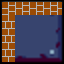
\includegraphics{assets/BarrierCorner/BarrierCorner01.png}
            % mit Sternchen * ohne Nummerierung
            \caption*{Beispielbild. Es gibt weiter Arten}
            \label{BarrierCornerFeld}
        \end{figure}
    \end{itemize}
    
    \item Seiten-Blockaden (BarrierSide)
    \begin{itemize}
        \begin{figure}[h]
            \centering
            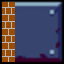
\includegraphics{assets/BarrierSide/BarrierSide1.png}
            % mit Sternchen * ohne Nummerierung
            \caption*{Beispielbild. Es gibt weiter Arten}
            \label{BarrierSideFeld}
        \end{figure}
    \end{itemize}
    
    \item Schwarzes-Loch (BlackHole)
    \begin{itemize}
        \begin{figure}[h]
            \centering
            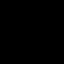
\includegraphics{assets/BlackHole/BlackHole.png}
            % mit Sternchen * ohne Nummerierung
            %\caption*{Beispielbild. Es gibt weiter Arten}
            \label{BlackHoleFeld}
        \end{figure}
    \end{itemize}
    
    \newpage
    \item Ziel-Punkte (Checkpoints)
    \begin{itemize}
        \begin{figure}[h]
            \centering
            
\includegraphics{assets/Checkpoints/Check1.png}
            % mit Sternchen * ohne Nummerierung
            \caption*{Beispielbild. Es gibt weiter Arten}
            \label{CheckpointFeld}
        \end{figure}
    \end{itemize}
    
    \item Fließband (ConveyorBelt)
    \begin{itemize}
        \begin{figure}[h]
            \centering
            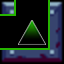
\includegraphics{assets/ConveyorBelt/ConveyorBelt12.png}
            % mit Sternchen * ohne Nummerierung
            \caption*{Beispielbild. Es gibt weiter Arten}
            \label{ConveyorBelt}
        \end{figure}
    \end{itemize}
    
    \item Express-Fließband (Express-ConveyorBelt)
    \begin{itemize}
        \begin{figure}[h]
            \centering
            
\includegraphics{assets/ExpressConveyorBelt/ExpressConveyorBelt23.png}
            % mit Sternchen * ohne Nummerierung
            \caption*{Beispielbild. Es gibt weiter Arten}
            \label{ConveyorBelt}
        \end{figure}
    \end{itemize}
    
    \newpage
    \item Zahnrad (Gear)
    \begin{itemize}
        \begin{figure}[h]
            \centering
            
\includegraphics{assets/Gear/Gear01.png}
            % mit Sternchen * ohne Nummerierung
            \caption*{Beispielbild. Es gibt weiter Arten}
            \label{ConveyorBelt}
        \end{figure}
    \end{itemize}
    
    \item Laser
    \begin{itemize}
        \begin{figure}[h]
            \centering
            
\includegraphics{assets/Laser/Laser00.png}
            % mit Sternchen * ohne Nummerierung
            \caption*{Beispielbild. Es gibt weiter Arten}
            \label{ConveyorBelt}
        \end{figure}
    \end{itemize}
    
    \item Drücker (Pusher)
    \begin{itemize}
        \begin{figure}[h]
            \centering
            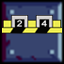
\includegraphics{assets/Pusher/Pusher01.png}
            % mit Sternchen * ohne Nummerierung
            \caption*{Beispielbild. Es gibt weiter Arten}
            \label{ConveyorBelt}
        \end{figure}
    \end{itemize}
    
    \newpage
    \item Reperaturfeld (RepairSite)
    \begin{itemize}
        \begin{figure}[h]
            \centering
            
\includegraphics{assets/Gear/Gear01.png}
            % mit Sternchen * ohne Nummerierung
            %\caption*{Beispielbild. Es gibt weiter Arten}
            \label{ConveyorBelt}
        \end{figure}
    \end{itemize}
    
    \item Backup-Feld (Checkpoint (Backup))
    \begin{itemize}
        \begin{figure}[h]
            \centering
            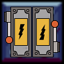
\includegraphics{assets/Checkpoint.png}
            % mit Sternchen * ohne Nummerierung
            %\caption*{Beispielbild. Es gibt weiter Arten}
            \label{ConveyorBelt}
        \end{figure}
    \end{itemize}
    
\end{itemize}

\chapter{Bedienung - User/Anwender}

    %
    Startet man das Spiel, so kann man im Startbildschirm auf Spiel starten klicken und somit die Mapauswahl, die Anzahl der Spieler (Jeder über 1 entspricht einem KI-Spieler) und der Map (Karte). Sollte keine expliziete Karte eingegeben werden, so wird automatisch die Standardkarte ausgewählt. \\
    Anschließend kann man wiederrum das Spiel beginnen.\\
    Im Spielbildschirm angekommen, sieht man links das Spielfeld (=board) und rechts eine Anzahl an buttons. Diese dienen zur Interaktion. So findet man im Schwarz unterlegten Bereich die Spielkarten des Spielers z.B.\\
    Für eine Spielanleitung bitte folgende Webseite konsulieren: \\
    \hypertarget{https://www.yumpu.com/de/document/read/27630938/roborallytm-regelbuch}{\url{https://www.yumpu.com/de/document/read/27630938/roborallytm-regelbuch}}
    %
    
\subsection*{Hinzufügen von neuen KIs per Schnittstelle}
    %
    Das manuelle einfügen von KIs erfolgt über das erstellen und importieren von selbst geschriebenen Klassen.\\
    Dabei müssen zwei Anforderungen erfüllt sein:
    \begin{itemize}
        \item Die KI-Klasse muss das AiInterface implementieren.
        \item Die KI-Klasse muss sich im htwk.mechawars.ai package befinden.
    \end{itemize}
    
    \newpage
    
    \noindent{Das} Hinzufügen erfolgt folgendermaßen:
    \begin{itemize}
        1.: Sicherstellen dass die oben genannten Vorraussetzungen erfüllt sind. \\
        2.: Importieren der KI in der Startupconfig.txt-Datei: \\
        \hspace*{10mm}´´Importing AI-Class-files syntax: 'AiImport: Class-file-Name'´´ (Auszug
        \hspace*{10mm}aus configreadme.txt). Man muss die Import-Zeile in der angegebenen Syn-
        \hspace*{10mm}tax in die Startupconfig.txt schreiben. \\
        3.: Festlegen der KI, die die Spieler nutzen werden: \\
        \hspace*{10mm}In der Zeile zum Festlegen der Starpositionen der Spieler, steht die letzte
        \hspace*{10mm}Zahl für den KI-modus des Spielers. \\
        \hspace*{10mm}Beispiel: playerposition: 1-3-3-2 \\
        \hspace*{15mm}Bedeutung: Spieler 1 startet an Position 3,3 und nutzt die zweite KI. \\
        \hspace*{15mm}Die Möglichkeiten für den KI-Modus sind wie folgt: \\
        \hspace*{18mm}0 - Keine KI: der Spieler bewegt sich nicht. \\
        \hspace*{18mm}1 - AiCardGeneration-KI: Standard-KI, die zufällig Karten aus einer
        \hspace*{24mm}Liste wählt. \\
        \hspace*{18mm}2-n - die Importierten KIs, in der Reihenfolge in der sie in Schritt 2
        \hspace*{18mm}importiert wurden. Wenn keine Angabe zum Spieler erfolgt, wird der
        \hspace*{18mm}Spieler keine KI besitzen. Wenn eine zu hohe Zahl angegeben wird,
        \hspace*{18mm}nutzt der Spieler die Standard-KI.
    \end{itemize}
    %

\chapter{Konsolen-Modus}
\subsection{Einrichtung}
    %
    Zunächst muss im Ordner \texttt{code} die gradlew.bat einmal ausgeführt werden. Anschließend kann in die Kommandozeile folgendes eingegeben werden:
    \begin{itemize}
        \item gradlew.bat desktop:dist
    \end{itemize}
    Dadurch wird im (neuerstellten) Unterordner \texttt{code/desktop/builds/libs} eine .jar Datei erstellt.
    %
    
\subsection{Starten}
    %
    Diese muss nun ausgeführt werden. Dazu ist der Befehl:
    \begin{itemize}
        \item java -jar desktop-1.0.jar
    \end{itemize}
    im entsprechenden Verzeichnis einzugeben.
    %

\subsection{Konfiguration(en)}
    %
    Für die Darstellung aller möglichen Konfigurationen muss in die Kommandozeile wiederrum die Eingabe erfolgen:
    \begin{itemize}
        \item java -jar desktop-1.0.jar -h
    \end{itemize}
    Das \textit{h} steht dabei für help (dt. = Hilfe). \\
    
    Sollte das Spiel im Konsolenmodus gestartet werden und der Befehl \textit{-w} eingetragen werden, so ist das spiel im Fullscreen-Modus (dt. = Vollbild).
    %


\end{document}
